\documentclass[12pt,a4paper,pdftex]{article}
\usepackage[left=25mm, right=25mm, top=20mm, bottom=25mm]{geometry}
\usepackage{graphicx}
\usepackage{amsmath}
% \usepackage{natbib}
\usepackage{biblatex}
\addbibresource{mothbib.bib} %Import the bibliography file
\usepackage{multirow}
\usepackage[inkscapelatex=false]{svg}
\usepackage[font=small,labelfont=bf]{caption}
\usepackage{epigraph}
\usepackage{placeins}
\usepackage[table,xcdraw]{xcolor}
\usepackage[breaklinks=true,bookmarks=true,bookmarksopen=true,pdfpagemode=UseNone,pdfstartview=FitH,colorlinks=true,citecolor=black,allcolors=black]{hyperref}
% \usepackage[section]{placeins}  % To keep floats in the sections in which they were included
\newcommand{\species}[1]{\textit{#1}}
\newcommand{\fig}[2]{(Fig.~#1~#2)}
\newcommand{\fileextension}[1]{\texttt{#1}}
\newcommand{\percent}[1]{#1~$\%$}
\newcommand{\relacs}[1]{\href{http://www.relacs.net}{#1}}



%%%%%%%%%%%%%%%%%%%%%%%%%%%%%%%%%%%%%%%%%%%%%%%%%%%%%%%%%%%%
% Titel- und Autoreninformation:
%%%%%%%%%%%%%%%%%%%%%%%%%%%%%%%%%%%%%%%%%%%%%%%%%%%%%%%%%%%%
\title{Moth Working Title}
\author{Nils Brehm} % Author name
\date{\today} % Datum (\today lassen oder durch richtiges Datum ersetzen)

\begin{document}
%%%%%%%%%%%%%%%%%%%%%%%%%%%%%%%%%%%%%%%%%%%%%%%%%%%%%%%%%%%%
% Cover:
%%%%%%%%%%%%%%%%%%%%%%%%%%%%%%%%%%%%%%%%%%%%%%%%%%%%%%%%%%%%
%\maketitle
\begin{titlepage}
	\begin{center}
		\vspace*{1cm}
		
		\begin{huge}
Discrimination of calls based on temporal information encoded by auditory receptor neurons of arctiid moths\\
		\end{huge}
		\begin{Large}
			\vspace{1cm}
			--- Can moths hear the difference?\\
		\end{Large}
	\end{center}
\end{titlepage}

%%%%%%%%%%%%%%%%%%%%%%%%%%%%%%%%%%%%%%%%%%%%%%%%%%%%%%%%%%%%
% Abstract:
%%%%%%%%%%%%%%%%%%%%%%%%%%%%%%%%%%%%%%%%%%%%%%%%%%%%%%%%%%%%
\newpage

% \section*{\centering{Abstract}}
\section*{Abstract}
Arctiid moths produce ultrasonic calls during courtship and for protection against predators. Every species has its own distinctive call pattern, which leads to a vast variety of different calls. Calls consist of single pulses, each one not longer than 1~ms. Such pulses can than be arranged in broader structures with intervals of around 1~--~100~ms.

Arctiid moths have a very simple ear with only two receptor cells with the same frequency tuning, and, therefore, are tone deaf. Thus, the temporal pattern of calls is, most likely, the salient characteristic that is perceivable for arctiid moths. Calls contain structures of several temporal scales and we could show that auditory receptor cells can resolve gaps longer than 2~--~5~ms, depending on the pulse duration. This makes it impossible for the nervous system to encode intervals between single pulses, but broader temporal structures are feasible. 

We could show that receptor cells can encode enough temporal information for a classification algorithm to discriminate between different species, successfully. Furthermore, an effective differentiation of moth and bat calls, which can mean the difference between life and death, is accomplished after just 50~ms. Based on those findings, we suppose that temporal call characteristics might play a more important role in courtship than thought before.   
\newpage

%%%%%%%%%%%%%%%%%%%%%%%%%%%%%%%%%%%%%%%%%%%%%%%%%%%%%%%%%%%%
% Introduction
%%%%%%%%%%%%%%%%%%%%%%%%%%%%%%%%%%%%%%%%%%%%%%%%%%%%%%%%%%%%
\section*{Introduction}
Arctiid moths are a divers subfamily in the Erebidae family (Lepidoptera/Noctuoidea) and are famous for their acoustic signals, pheromonal system and interactions with bats. Most species posses modified thoracic metepisternum on the third  pair of hind legs, called tymbals. With this organ, arctiid moths can produce ultrasonic pulses. The tymbal organ has a stiff membrane and is filled with air \cite{blest1963, fullard1977, fullard1990}. Attached to the membrane are three different muscles that are innervated by a branch of the metathoracic leg nerve (IIIN2a) and receive signals from a cluster of 5--9 motor neurons \cite{nuesch1957, fullard1992}. The contraction of those muscles leads to a buckling in of the whole organ that moves from dorsal to ventral. After the muscles relax again, the movement reverses and the tymbal passively buckles out again \cite{blest1963}. Many species have a striated band on top of the tymbal membrane (microtymbals or striae). Those striae act like single instruments and each produces a single pulse \cite{blest1963, fullard1977, fullard1990, weller1999}. 
The frequency components of each stria sound can change from stria to stria. In many species those single pulses are combined to a series of pulses. Such a series is called a call and contains all pulses that are generated during an activation phase of the tymbal. In this phase, the muscles are contracting and relaxing periodically with only short intervals. Thereby the buckling in and out of striae moves along the dorsal-ventral axis of the tymbal, producing pulses actively and passively \cite{corcoran2010}. This leads to the typical temporal structure of moth calls, since in many species this movement along the tymbal is smooth. This means that a call is build up of an active and passive pulse train, due to the active and passive buckling of the tymbal organ. If some of the pulses have different spectral components, this can result in 'melodies' within a call. Furthermore the tybmals on both sides of the body can be activated in almost synchrony, anti-phase or with some amount of lag \cite{fullard1977}. Depending on the phase of both tymbals the resulting call can show remarkable interferences. Most of the arctiid moths produce species specific calls that are inimitable enough to be called an acoustic fingerprint (Philipp Klein, personal communication). 

Of course moths are capable of hearing those calls as well. How precise they can perceive such signals is, however, still not absolutely clear. The ear of acrtiid moths is a typical insect tympanal organ and is one of the simplest ears in the animal kingdom, even for insects. It is positioned right between the thorax and abdomen on both sides of the animal. A thin membrane is spanned over several air filled chambers. In the center of this membrane the dendrites of two receptor cells (A1 and A2) are attached to it \cite{yager1999}. Via the acoustic nerve (IIIN1b), the axons of those cells project to the thoracic Pteroganglion \cite{paul1973}. The receptor cell type is descended from Chordotonal organs, Type I mechanoreceptors that are distributed over the entire body of many insects \cite{miller2001, yack2004}. Auditory receptor cells are excited by ultrasonic sound, most strongly for frequencies of 20--60~kHz \cite{fullard1988, yager1999, terhofstede2013, nakano2014}. Both A1 and A2 show the same frequency tuning, although A2 is 20~dB~SPL less sensitive \cite{miller2001}. This means that moths are tone deaf and a discrimination between different frequencies is not possible, since the animals cannot determine if increasing neuronal activity is due to intensity or frequency \cite{roeder1966, terhofstede2013}. Additionally to the A1 and A2 cells, another receptor, the B cell was found in the ears of arctiid moths. However the cell does not respond to sound \cite{fullard2003} and is supposed to have some function in proprioception, like encoding physical stress within the tympanal organ \cite{waters2003}. 

The evolution of moth ears is one of the classical examples of an arms race in biology \cite{hofstede2016}. The prevalent hypothesis is that ears in moths have evolved to detect bats hunting with the help of their echolocation system \cite{roeder1961detection, miller2001, ratcliffe2009, conner2012}. Insectivorous bats emit calls in the ultrasonic spectrum to detect and catch insects during the night \cite{schnitzler2001}. Those calls can be detected by moths and triggers several defensive behaviors. Exposed to bat calls during flight, moths tend to show an evasive behavior. If the bat is far away, moths fly in the opposite direction. In close range, however, moths start to fly in an erratically fashion, making it hard to predict where it is going to move \cite{roeder1961detection, acharya1999}. Some moths show an acoustic response, as well. If the bat is close to the moth and emits high intensity echo location calls, some moth species respond by emitting sound. This defensive reaction can prevent the bat from catching it. Why the bat is distracted is not yet clarified to the last detail. Either bats are jammed by the moth calls, i.e. the bat's nervous system is overloaded and location is temporally not functioning \cite{corcoran2010, corcoran2011, conner2012}. Or bats are just startled by the sudden noise and therefore fail to catch the moth \cite{fullard1977}. Another possibility is that bats can recognize different moth calls and learn which of them taste awful. Many arctiid species feed on pyrrolizidine alkaloids (PA) bearing plants \cite{boppre2011, ratcliffe2005}. PAs are toxic and lead to an unpleasing taste. Bats can make this association and avoid distasteful moths, which can be interpreted as an acoustic version of aposematism \cite{eckrich1990chemical, hristov2005, miller2001}. 

Beside the role of moth calls as a defensive strategy against bats, sound production is also involved in courtship and mating. Several authors could show that acoustic signals are part of the courtship in arctiid moths and that it is somehow important for successful mating \cite{sanderford1990, simmons1996, sanderford1998}. In one case, however, acoustic signals were only important in the absence of chemical cues \cite{conner1987}. On the other hand, \cite{weller1999} found two species that had completely lost pheromonal courtship and only rely on acoustic signals. Those signals could initially evolved for protection against predators, but than secondarily started to play an important role in courtship \cite{simmons1996, phelan1997evolution, weller1999}. Concerning the involvement of acoustic communication in mating it is evident that the moth's nervous system must be able to process the information content of calls. The animal has to recognize conspecfic calls and differentiate between mating signals and other sources of sound like calls of other species or bats, and environmental noise. The primary information on which such a task can be based upon comes from the neuronal activity of the moth's auditory receptor cells. If acoustic signals play an important role in intraspecific communication, the difference of calls encoded in the receptor's spike trains must be distinct enough for the nervous system to act appropriately. 

In this study we investigate if there is sufficient information in the spike trains of receptor cells in response to different moth and bat calls. We suppose that the temporal structure of calls is the key property for this task. Therefore we first examine the temporal and spectral resolution of the moth's auditory neurons and than test how reliable a classification of moth call, based spike trains, can be.
\newpage

%%%%%%%%%%%%%%%%%%%%%%%%%%%%%%%%%%%%%%%%%%%%%%%%%%%%%%%%%%%%
% Methoden
%%%%%%%%%%%%%%%%%%%%%%%%%%%%%%%%%%%%%%%%%%%%%%%%%%%%%%%%%%%%
\section*{Methods}
\subsection*{Animals}
Three moth species (\species{Carales astur} and \species{Estigmene acrea} originated from Costa Rica and \species{Creatonotos transiens} originated from Indonesia) of the subfamily Arctiinae of both sexes were used for electrophysiological experiments at the University of T{\"u}bingen. Larvae were reared on semiartificial diet modified after \cite{bergomaz1986} and kept in plastic boxes at $24\pm2$ $^{\circ}$C, under artificial light (12:12 hrs) at the University of Freiburg. All species readily mated in gauze cages. Adult animals were kept in plastic boxes permeable to air and supplied with sugar water. Data from male and female moths were pooled. No difference between sexes could be found and neural auditory thresholds are indistinguishable
\cite{terhofstede2013}.        

\subsection*{Electrophysiology}
% \subsubsection{Preparation}
For recording the neural activity of the auditory nerve (3N1 after \cite{nuesch1957}) a modified approach by \cite{roeder1957} was used. Animals were dealated and the dorsal side of the thorax was descaled. Then the legs were removed and the animal was fixated on a table ventral side up using insect wax. The thorax was cut open along the mid-ventral line, whereby exposing the pterothoracic ganglion. The thoracic cavity was flooded with saline and the tympanal branch of the nerve 3N1 was hooked with a silver hook electrode. This branch consist of two auditory receptor axons (A1 and A2) and projections of a proprioception cell (B cell), which is not excited by acoustic stimuli. Another silver electrode was placed lateral in the thorax, serving as a reference.   

% \subsubsection{Data Acquisition}
All signals recorded from the auditory nerve were amplified and filtered with two coupled extracellular amplifiers (EXT-10-2F and DPA-2FX, npi electornics Tamm) with a total gain of 10k. The low and high pass filters were set to 3~kHz and 400~Hz, respectively. The amplified signal was then recored using \relacs{RELACS} \footnote{http://relacs.sourceforge.net/index.html}. All experiments were done in a sound proof chamber with no lighting. Spikes were detected using a dynamic amplitude threshold. B~cell spikes had much higher amplitudes and a regular firing pattern and, based on that, were rejected from the analysis. A1 and A2 spikes could not be discriminated and were treated together as if belonging to one unit. 


\subsection*{Stimuli}
For presenting acoustic stimuli, a speaker (TG30) connected to the recording computer via an audio amplifier (ATN-01 M, , npi electornics Tamm) was placed into the sound proof chamber with a distance of 40~cm to the preparation. The speaker was calibrated using an ultrasonic microphone (Gras). This procedure was repeated for several times to make sure the calibrations stayed valid. All stimuli were played back with \relacs{RELACS}.

\subsubsection*{Intensity and frequency tuning}
To determine the frequency tuning of the receptors, pure tone pulses (sinusoidal sound waves) with a duration of 20~ms to 50~ms were presented. The carrier frequency was varied in 10~kHz steps between 10~kHz and 100~kHz. Stimulus intensity was increased in 3~dB~SPL steps from 20~dB~SPL to 90~dB~SPL.

\subsubsection*{Temporal resolution}
Moth ears were exposed to amplitude modulated sine waves with a carrier frequency of 50~kHz. Amplitude modulation was done by using a rectangular function, which sets the intensity to either 0~dB~SPL or 80~dB~SPL and therefore producing a pulsed stimulus with particular gaps in between. The pulse duration was either 5~ms or 10~ms and the period was chosen, so that the gap between two successive pulses was 0~ms to 20~ms long. A period of 30~ms with a pulse duration of 10~ms corresponded to a gap of 20~ms. Every gap trial was repeated 20 times. In addition, artificial moth pulses with varying intervals were presented to the animals. Moth pulses were approximated by damped sine waves with a carrier frequency ($f_{i}$) of 50~kHz, a damping constant ($\tau$) of 0.1~ms and 0.4~ms and a single pulse duration of 0.5~ms and 2~ms, respectively.

\begin{equation}
\label{eq:DampedSine}
Pulse(t) = \sum_{i}^{N} a_i~ sin(\omega_i t) ~e^{-\frac{t}{\tau}}~~,~~~~ \omega_i = 2 \pi f_i  
\end{equation}

\subsubsection*{Moth and bat calls}
The possibility of discriminating different moth and bat calls by looking at the neural response (i.e. spike trains) was tested by using playbacks of moth and bat single calls and call series. A single moth call consisted of one active and one passive pulse train. In a call series, this acoustic unit is repeated several times yielding a longer stimulus time and adding coarser temporal patterns. Every stimulus was presented 20 times at a sound pressure level of 80~dB~SPL. To obtain those calls, animals were fixed between the index finger and thumb. By gently squeezing the animal, it started emitting calls. Those calls were recorded, using a microphone (Knowles Electronics, FG-23329) sensitive to ultrasound, with a sampling rate of either 256~kHz or 480~kHz. Calls that are recored with this method are not distinguishable from calls elicited with play backs of bat calls \cite{barber2006, corcoran2010}.

Many calls did differ in their duration. Therefore we corrected for this difference by extending all calls to the same length. This was done by repeating the particular spike train response, i.e. adding the whole spike train successively with a gap of 10~ms for single calls and 50~ms for call series. Spike trains that were treated this way were called 'extended'. It is important to emphasize that we did not repeat the acoustic stimuli, but the spike trains produced by the receptor cells in response to the untreated calls.


\subsection*{Analysis}
Recording data was stored in the \href{https://github.com/G-Node/nix/wiki}{nix} \footnote{https://github.com/G-Node/nix/wiki} (neuroscience information exchange) format and analyzed using the programming language Python (v3.5).
 
\subsubsection*{Intensity and frequency tuning}
We used kernel density estimations with a gaussian kernel to compute firing rates. Based on the firing rate a threshold was found by fitting a Boltzmann function to the data (\ref{eq:Boltzmann}), resulting in a sigmoidal function \cite{benda2008}.
\begin{equation}
\label{eq:Boltzmann}
f(I) = f_{min} + \frac{(f_{max}-f_{min})}{1+e^{-k(I-I_0)}}
\end{equation}
At $I_{0}$, which is half way between the minimum ($f_{min}$) and the maximum ($f_{max}$) values, this function can be approximated by a straight line.

The intensity value at which the tangent at $I_{0}$ crosses the minimum ($f_{min}$) value is defined as the threshold (\ref{eq:Threshold}),  
\begin{equation}
\label{eq:Threshold}
Threshold = I_{0} - \frac{2}{k}
\end{equation}
where $k$ is a constant value, corresponding to the slope of the tangent.
This method of finding a threshold is much more sophisticated than just setting it to an arbitrary spike count which is quite common in the moth literature, yet still yielding similar results.


\subsubsection*{Temporal Resolution}
For measuring the phase locking of spikes to the stimulus period, we computed the vector strength (VS). 
\begin{equation}
\label{eq:VS}
VS = \left|\frac{1}{n} \sum_{j=1}^{n}e^{i\omega t_j}\right|
\end{equation}
All spike times of one trial ($t_{j}$) are put on a unity circle in reference to the stimulus period~$T$, which is included into the angular frequency $\omega = \frac{2\pi}{T}$. The absolute value of the average vector is then called the vector strength. It falls between 0, no locking at all, and 1, indicating perfect locking \cite{vanhemmen2013}. 
The VS for a range of periods (0 to 50~ms) was computed for every single spike train and than averaged over trials (second order VS spectrum, \cite{sinz2017a}). 
If there is a particular locking to a specific stimulus period the VS spectrum function peaks. To determine if this VS peak yields an significant effect we compared it to the 95 percentile of the bootstrapped VS distribution of a Poisson model neuron. The firing rate was equal to the mean firing rate of the recorded cell and the Poisson spike trains only showed a synchronization pattern by chance. 

\subsubsection*{Spike train distances}
\label{spiketraindistances}
We quantified the  differences between spike trains with the Van Rossum distance \cite{rossum2001}, which replaces every spike with a exponential function.
\begin{equation}
\label{eq:VR}
f(t) =  \sum_{i}^{M} H(t-t_i)~e^{\frac{-(t-t_i)}{\tau}}
\end{equation}
$H$ is an Heaviside step function.
\begin{equation}
\label{eq:H}
H(x) = \left\{
\begin{array}{ll}
0 & \quad x < 0 \\
1 & \quad x \geq 0
\end{array}
\right.
\end{equation}
and $\tau$ is the time constant of the exponential function, determining how fast the function decays.
This time constant can be freely chosen so that the experimenter can investigate different time scales that might be biological interesting.
For every comparison between two spike trains the continuous functions ($f(t)$) are subtracted, squared, summed and normalized by $\tau$. 
\begin{equation}
\label{eq:VRD}
D_{VR}(f,g) = \frac{1}{\tau} \int_{0}^{\infty}[f(t)-g(t)]^2 dt
\end{equation}
This yields a single distance value for every comparison. If $\tau$ is set to a very small value, the Van Rossum distance counts noncoincident spikes. If set to a large value the difference in total spike count is measured.

\subsubsection*{Spike train classification.}
To investigate if a discrimination between calls, just by looking at the spike trains, is possible, a modified procedure by \cite{machens2003} was applied. For every call stimulus 20 repetitions were recorded. Out of this 20 spike trains, one was selected as a template. This template was then compared to all the other spike trains of the same call, and to all other call stimuli, but not with itself. For 20 different calls this yields a number of 399 comparisons. The spike train that had the smallest distance to the template was treated as the best match. By looking at the corresponding calls, to which this matched spike train belonged, a classification could be conducted. This procedure was repeated for all the other call stimuli and then bootstrapped ten times. The resulting algorithm seems to be a good compromise between doing all possible combinations and tolerable computing time.

\subsubsection*{Poisson trains}
The duration of moth calls was different between the single species. To have a better idea how the spike train distance metrics, used in this study, behave if there is no other information present than the total spike train duration, we computed the distances for groups of Poisson trains and run the classification algorithm on them.
For the Van Rossum metric, the expected distance can be found analytically (eq. \ref{eq:Poisson_Estimated_VR} from \cite{rossum2001}). 
\begin{equation}
\label{eq:Poisson_Estimated_VR}
D^{2} = pT~~,~~~~~~~p:~firing~rate,~T:~total~duration
\end{equation}
This means that the Van Rossum distance for Poisson trains only depends on the firing rate and the total spike train duration, and is independent of $ \tau $. However, $ \tau $ strongly influences how large the variance of the metric is. The Van Rossum distance with large $ \tau $ values measures the difference in total number of spikes. Whereas small $ \tau $ values correspond to  a non-coincident counter. The difference in total spike count varies more than the number of non-coincident spikes \cite{rossum2001}. Therefore the variation among distances computed with large $ \tau $ values is significantly higher \cite{rossum2001}. 

\newpage
\subsection*{Discrimination of moth and bat calls}
\label{MvsBMethods}
Discrimination between different calls is a quite sophisticated task. A more fundamental skill is to classify moth and bat calls. The observer of spike trains is confronted with a task that can be broken down to a 'yes' or 'not' task. When an observer looks at a spike train, it can either say, it is the response to a moth or to a bat call. Table \ref{tab:yesno} shows the classification of decisions based on the Signal Detection Theory. Converting the hits and false alarms to rates, the sensitivity index $d'$ (d prime) can be computed by performing a subtraction of the z-transformations of those rates.
\begin{equation}
\label{eq:dprime}
d' = z(hit~rate) - z(false~alarm~rate)
\end{equation}


\begin{table}[h]
	\centering
	\caption{Classification of decisions based on the Signal Detection Theory. Bat calls are treated as signals and moth calls as noise in a 'yes' or 'no' task. Ground truth: the stimulus that was presented to the animal. Decision: The outcome of the classification algorithm based on spike trains.}
	\setlength{\tabcolsep}{10pt} % Default value: 6pt
	\renewcommand{\arraystretch}{1.5} % Default value: 1
	\label{tab:yesno}
	\begin{tabular}{llcc}
		&                                                   & \multicolumn{2}{c}{\cellcolor[HTML]{C0C0C0}\textbf{Ground truth}} \\
		&                                                   & \cellcolor[HTML]{C0C0C0}Bat     & \cellcolor[HTML]{C0C0C0}Moth    \\ \cline{3-4} 
		\multicolumn{1}{c}{\cellcolor[HTML]{C0C0C0}{\color[HTML]{000000} }}                                    & \multicolumn{1}{c|}{\cellcolor[HTML]{C0C0C0}Bat}  & Hit                             & False alarm                     \\
		\multicolumn{1}{c}{\multirow{-2}{*}{\cellcolor[HTML]{C0C0C0}{\color[HTML]{000000} \textbf{Decision}}}} & \multicolumn{1}{c|}{\cellcolor[HTML]{C0C0C0}Moth} & Miss                            & Correct rejection              
	\end{tabular}
\end{table}
\FloatBarrier

%%%%%%%%%%%%%%%%%%%%%%%%%%%%%%%%%%%%%%%%%%%%%%%%%%%%%%%%%%%%
% Results
%%%%%%%%%%%%%%%%%%%%%%%%%%%%%%%%%%%%%%%%%%%%%%%%%%%%%%%%%%%%
\newpage
\section*{Results}
\subsection*{Call structure of moth calls}
All moth calls used in this study are listed in Tab.~\ref{tab:SC} and Tab.~\ref{tab:CS}. We differentiated between single calls and call series. The minimal unit is the single pulse. Those pulses are then further arranged in one call. A call series is defined as several calls in a row. Fig.~\ref{fig:01}(A, B, C) gives an overview of the different structures of a moth call series.

\subsubsection*{Single pulses}
A single pulse can be described by a damped sine wave \fig{\ref{fig:01}}{C} and pulse duration was defined as the time between pulse onset and crossing of a threshold that was set according to the standard deviation of the noise. In all calls used in this study it ranged from 0.1~ms to 0.6~ms \fig{\ref{fig:01}}{D}. Thus all pulses produced by the tymbals of different moths were shorter than one millisecond. A duration that is in the same scale of action potentials. Active and passive pulses did not differ in duration in the same call. The interval between two pulses (IPI) was mainly below 5~ms \fig{\ref{fig:01}}{E}. The fundamental frequency of the single pulses varied around 15~kHz to 65~kHz \fig{\ref{fig:01}}{F}, and the frequency for active and passive pulses in the same call did not differ decisively.

\subsubsection*{Single calls}
Intervals between the active and the passive pulse trains (ITI) varied from 2~ms up to 80~ms \fig{\ref{fig:01}}{H}. The call duration ranged around 20~ms to 180~ms \fig{\ref{fig:01}}{I}. Moth calls were chosen by the experimenter to have the same number of active and passive pulses and only three calls did differ in this aspect. The number of active and passive pulses was between 1 to 24 pulses \fig{\ref{fig:01}}{G}.

\begin{table}[h]
	\centering
	\caption{Single moth calls used in this study. Shown are the duration, inter train interval (IT) and number of active and passive pulses. Some of the species could not be determined with \percent{100} accuracy and were labeled with an internal code. The recording ID corresponds to the call IDs shown in all figures.}
	\setlength{\tabcolsep}{6pt} % Default value: 6pt
	\renewcommand{\arraystretch}{1.5} % Default value: 1
	\label{tab:SC}
	\begin{tabular}{llcccc}
		\rowcolor[HTML]{EFEFEF} 
		ID & {\color[HTML]{000000} Species}     & \multicolumn{1}{c}{\cellcolor[HTML]{EFEFEF}Duration } & \multicolumn{1}{c}{\cellcolor[HTML]{EFEFEF}ITI} & \multicolumn{1}{l}{\cellcolor[HTML]{EFEFEF}Active} & \multicolumn{1}{l}{\cellcolor[HTML]{EFEFEF}Passive} \\
		\rowcolor[HTML]{EFEFEF}
		& & \multicolumn{1}{c}{\cellcolor[HTML]{EFEFEF}[ms]} & \multicolumn{1}{c}{\cellcolor[HTML]{EFEFEF}[ms]} & \multicolumn{1}{l}{\cellcolor[HTML]{EFEFEF}Pulses} &
		\multicolumn{1}{l}{\cellcolor[HTML]{EFEFEF}Pulses} \\ \hline
		
		0            & BCI1062                            & 17.10                                                & 4.79                                            & 7                                                         & 7                                                          \\
		1            & Aclytia gynamorpha          & 36.79                                                & 5.44                                            & 24                                                        & 24                                                         \\
		2            & Agaraea semivitrea          & 25.72                                                & 8.58                                            & 7                                                         & 7                                                          \\
		3            & Carales astur              & 75.64                                                & 7.89                                            & 12                                                        & 12                                                         \\
		4            & Chrostosoma thoracicum       & 27.25                                                & 5.43                                            & 5                                                         & 5                                                          \\
		5            & Creatonotos transiens                  & 11.64                                                & 11.64                                           & 1                                                         & 1                                                          \\
		6            & Elysius conspersus           & 148.45                                               & 28.04                                           & 10                                                        & 11                                                         \\
		7            & Epidesma oceola              & 45.32                                                & 23.76                                           & 6                                                         & 6                                                          \\
		8            & Eucereon appunctata          & 32.75                                                & 9.50                                            & 13                                                        & 12                                                         \\
		9            & Eucereon hampsoni            & 18.94                                                & 3.43                                            & 11                                                        & 11                                                         \\
		10           & Eucereon obscurum            & 34.83                                                & 9.01                                            & 14                                                        & 14                                                         \\
		11           & Hypocladia restriata                        & 183.47                                               & 89.49                                           & 11                                                        & 11                                                         \\
		12           & GL116                        & 42.61                                                & 17.93                                           & 5                                                         & 5                                                          \\
		13           & Hypocladia militaris         & 54.07                                                & 6.13                                            & 9                                                         & 9                                                          \\
		14           & Idalu fasciipuncta           & 63.95                                                & 25.88                                           & 5                                                         & 5                                                          \\
		15           & Idalus daga                & 21.02                                                & 4.73                                            & 18                                                        & 18                                                         \\
		16           & Melese sp.             & 26.59                                                & 5.44                                            & 12                                                        & 12                                                         \\
		17           & Neritos cotes               & 23.61                                                & 3.12                                            & 10                                                        & 10                                                         \\
		18           & Ormetica contraria peruviana & 38.08                                                & 1.08                                            & 7                                                         & 11                                                         \\
		19           & Syntrichura sp.                  & 56.23                                                & 12.06                                           & 12                                                        & 
		12   \\ \hline 
		& Median & 35.81 &	8.24 &	10 &	11 \\
		& Mean & 48.83 &	14.28	& 9.84 &	10.05 \\
		& Standard Deviation & 43.55 &	19.36 &	5.12	& 5.06 \\
		& Minimum & 11.64	& 1.08 &	1	& 1 \\
		& Maximum &183.47	& 89.49	& 24 &	24
		
		
		
		                                                    
	\end{tabular}
\end{table}

\subsubsection*{Call series}
In nature, calls rarely occur isolated, but are repeated in call series. The call series is therefore the natural signal of arctiid moths. The duration of call series used in this study ranged from 0.14~s to 3.99~s (Fig.~\ref{fig:01}~{I}~and~Tab.~\ref{tab:CS}). About half of the call series were not longer than 1~s. The number of pulses emitted during this time did differ between species. The pulse rates (pulses per second) had a minimum of 12~Hz and a maximum of 795~Hz (Tab.~\ref{tab:CS}). Moreover, calls are not homogeneously distributed in call series. Many species tend to cluster calls in packages with short intervals between the calls in one package and much longer intervals between packages. Hence, the acoustic signal emitted by arctiid moths shows a modular composition. If we sort those modules in increasing duration we then have the single pulse and the inter pulse interval, the pulse train and the inter pulse train interval, the call, the package of calls and the call series. This raises many different temporal scales a receptor neuron could be tuned to \fig{\ref{fig:01}}{A}. 
 
\begin{table}[p]
	\centering
	\caption{Moth call series used in this study. Shown are the duration, number of pulses and pulse rate of moth call series in seconds. Some of the species could not be determined with \percent{100} accuracy and were labeled with an internal code. The recording ID corresponds to the call IDs shown in all figures.}
	\setlength{\tabcolsep}{10pt} % Default value: 6pt
	\renewcommand{\arraystretch}{1.5} % Default value: 1
	\label{tab:CS}
\begin{tabular}{llccc}
	\rowcolor[HTML]{EFEFEF} 
	ID & {\color[HTML]{000000} Species} & \multicolumn{1}{l}{\cellcolor[HTML]{EFEFEF}Duration {[}s{]}} & \multicolumn{1}{l}{\cellcolor[HTML]{EFEFEF}Pulses} & \multicolumn{1}{l}{\cellcolor[HTML]{EFEFEF}Pulse rate {[}Hz{]}} \\ \hline
	0  & A7838                          & 0.22                                                         & 84                                                 & 382                                                             \\
	1  & BCI1348                        & 0.14                                                         & 27                                                 & 193                                                             \\
	2  & Chrostosoma thoracicum         & 3.5                                                          & 350                                                & 100                                                             \\
	3  & Creatonotos transiens          & 2.04                                                         & 26                                                 & 13                                                              \\
	4  & Eucereon appunctata            & 1.03                                                         & 108                                                & 105                                                             \\
	5  & Eucereon hampsoni              & 0.96                                                         & 92                                                 & 96                                                              \\
	6  & Eucereon maia                  & 0.76                                                         & 12                                                 & 16                                                              \\
	7  & Hypocladia restriata           & 0.22                                                         & 23                                                 & 105                                                             \\
	8  & Hyaleucera erythrotelus        & 2.97                                                         & 42                                                 & 14                                                              \\
	9  & Hypocladia militaris           & 1.52                                                         & 105                                                & 69                                                              \\
	10 & Eucereon appunctata            & 0.17                                                         & 88                                                 & 518                                                             \\
	11 & PP612                          & 2.76                                                         & 505                                                & 183                                                             \\
	12 & PP643                          & 0.4                                                          & 33                                                 & 83                                                              \\
	13 & Saurita sp.                    & 0.41                                                         & 44                                                 & 107                                                             \\
	14 & Uranophora leucotelus          & 0.47                                                         & 292                                                & 621                                                             \\
	15 & Carales astur                  & 1.87                                                         & 215                                                & 115                                                             \\
	16 & Melese sp.                     & 3.99                                                         & 795                                                & 
	199           \\ \hline
	& Median & 0.96	& 88	& 105 \\
	& Mean & 1.38	& 167.12 &	171.71 \\
	& Standard Deviation & 1.26	& 212 &	174.50 \\
	& Minimum & 0.14	& 12	& 13 \\
	& Maximum & 3.99 &	795	& 621
	
	
	                                                
\end{tabular}
\end{table}
\FloatBarrier

\subsection*{Intensity and frequency tuning}
First, we investigated how the moth's auditory receptor cells responded to sine waves that differ in intensity and frequency. Based on neuronal activity measurements, we computed the respective tuning curves for \species{Carales astur} and \species{Estigmene acrea}.  

\subsubsection*{Intensity tuning}
With increasing intensity at a fixed frequency the firing rate of the auditory receptor cells increased in a sigmoidal fashion that can be well described by a Boltzmann function \fig{\ref{fig:02}}{A}. By extrapolating the tangent at $I_{0}$, a threshold can be defined by the intersect of that tangent and the minimum ($f_{min}$) value. This is indicated by the red line in Fig.~\ref{fig:02}{A} for a stimulus frequency of 20~kHz and 85~kHz.  

\subsubsection*{Frequency tuning}
By taking all intensity threshold values for different frequencies together, an audiogram can be plotted. This audiogram can differ between species. Both audiograms of \species{Carals astur} and \species{Estigmene acrea} have a broad frequency tuning, reaching from 10~kHz to 100~kHz, but \species{Carales astur} \fig{\ref{fig:02}}{D} was tuned more towards the high frequencies, whereas \species{Estigmene acrea} has a more equal distribution over the same frequency range. For \species{Estigmene acrea} two different stimulus durations were tested. Both yielded nearly the same audiogram curves \fig{\ref{fig:02}}{C}.
 
\subsubsection*{Matched filter}
Moths are naturally exposed to more complex sounds coming from other animals. To get a better biological interpretations of the audiograms, we compared them with the power spectrum of their own calls and several bat calls that were used in this study \fig{\ref{fig:02}}{B}. Both calls of \species{Carales astur} and \species{Estigmene acrea} have a broad power spectrum. The power spectrum of \species{Estigmene acrea} is flat with a drop at around 60~kHz. That of \species{Carales astur} is bimodal with the two peaks at around 30~kHz and 70~kHz. Taking all bat calls together, the power is high between 20~kHz and 90~KHz. Above and below this range power drops drastically.

\subsection*{Temporal resolution}
The temporal structure of moth calls is one of the major properties a discrimination can be based on. Therefore we recorded the response of auditory receptor cells of \species{Estigmene acrea} to rectangular stimuli and model pulses with different gap length.

\subsubsection*{Gap detection}
For gap length as long as 20~ms the firing rate followed the stimulus precisely and approximated a sinusoidal curve with same temporal structure as the stimulus (SuppFig???). However, with decreasing gap size this pattern was becoming more irregular. Therefore, the exact matching between firing rate and stimulus was lost at shorter gaps (SuppFig???). 
When exposing the animal to a constant pure tone with no gaps in between, the temporal pattern vanished completely and the response resembles a typical adaptation to constant sounds (SuppFig???).
The inter spike interval (ISI) histogram of the response to long gaps is bimodal. With one peak around 5~ms and the other at 25~ms. Those two peaks corresponded to the mean firing rate and the stimulus gap size, respectively. The ISI distribution for such gaps was clearly different from a Poisson ISI distribution with its typical exponential decay (SuppFig???). 

With decreasing gap size, the bimodal distribution turned into a monomodal one, because the stimulus period approached the firing rate. Here, the encoding would switch from a rate code to a temporal one. Instead of the firing rate following the stimulus, single spikes locked to the stimulus period. The phase locking between stimulus period and receptor response was quantified using the vector strength approach. The vector strength spectrum peaks at stimulus periods to which the neural response is locked. If this peak is above the 95~percentile range of a Poisson model neuron, the locking is significant (SuppFig???). 

Beside the strong locking to the stimulus period, we could observe high vector strength values for harmonics of the stimulus period and mean firing rate, as well. For a long gap duration, spikes were locked to the first half of the stimulus phase, shifting to the end of the phase for decreasing gap sizes. When there were no gaps in the stimuli, there was no specific locking to any part of the phase, resembling more the Poisson neuron model (SuppFig???).

\subsection*{Encoding of moth calls}
\label{mothcalls}
We recorded the response of auditory receptor cells to different moth call series. To investigate if calls can be classified by looking at the spike trains we used a classification algorithm based on spike train distances.
\subsubsection*{Spike train classification}
Spike trains were classified by computing the pairwise spike train distance and matching those with the smallest distance values. The Van Rossum distance has the advantage of comparing spike trains at different temporal resolutions by choosing a particular value for the time constant~$\tau$ of the exponential (eq.~\ref{eq:VR}) that converts spike times to a continues function. Fig.~\ref{fig:03}~A shows the spike train matching for moth call series after 1~s. A low $\tau$ value of 1~ms led to incorrect matching. By increasing $\tau$ to 10~ms the matching improved clearly. A further increase to 1000~ms, however, did not improve the matching \fig{\ref{fig:03}}{A}. 

To control for the different duration of calls, we extended all spike trains to the same length.
However, in the case of a presentation time of 1~s, the extension of spike trains only changed spike train matching matrix slightly.
To see what temporal resolution and presentation time yield the best performance in classification of different moth call series, we computed the classification with different $ \tau $ values for the Van Rossum metric. We found that the performance of classification depended on the temporal resolution. At $5-100$~ms , \percent{$70-80$} of the calls were classified correctly when taking at least a spike train duration of 300~ms into account. Extended spike trains showed the same performance at 300~ms for a temporal resolution of $10-80$~ms. However, after around 1~s the performance drastically decreased again to values of around \percent{50} \fig{\ref{fig:03}}{B}. 

\subsubsection*{Poisson trains}
Spike times that are determined by a Poisson process are a valuable tool to control for classification algorithms based on spike train distances, since the pattern of the spike times is random in its nature and has a fixed firing rate.
To have a comparable set of data, we performed a classification algorithm on 17 groups, all with different total duration, equal to the different duration of the moth call series (Tab.~\ref{tab:CS}). Each group had 20 trials (Poisson spike trains with a firing rate of 100~Hz). Furthermore there was a set of 17 groups that all had a duration of 2~s, again each with 20 trials each. The performance of the Van Rossum based classification for the groups with different durations is shown in Fig.~\ref{fig:03}~B. After 1~s around \percent{50} of the spike trains were correctly classified. Beyond 2~s it increased to \percent{75}. The optimal temporal resolution ($ \tau $) window was between 10~ms and 300~ms. With a firing rate of 100~Hz, 10~ms corresponds to the inter spike interval of the Poisson trains.

\subsection*{Moth vs. bat calls}
\subsubsection*{Classification based on percentage}
Moth and bat calls were analyzed based on the Van Rossum metric, as described before. However, this time the classification algorithm concentrated on discriminating between bat and moth calls. Therefore, the classification was based on the two broader groups, moths and bats, and not on single species. 
Fig.~\ref{fig:03}~C~ shows the percentage of spike trains classified as moth calls based on the Van Rossum distance with a temporal resolution ($ \tau $) of 1~ms, 10~ms and 1000~ms. 
When the temporal resolution was as small as 1~ms, the difference between moth and bat calls was not present. Interestingly, for the unchanged call series most calls were classified as bat, whereas extended calls were mostly classified as moth \fig{\ref{fig:03}}{C: top panel}. 
Increasing the temporal resolution to 10~ms led to a separation between moth and bat calls. 
After 200~ms most of the original bat calls were classified as such. The original moth calls, however, showed more 'wrong' classification. Some responses (spike trains) were classified as bat calls instead of moth calls. Furthermore, after 200~ms the percentage of moth calls was independent of spike train duration. Extended spike trains showed a higher success in matching moth calls correctly, however, bat calls were misinterpreted as moth calls more often \fig{\ref{fig:03}}{C: middle panel}. Increasing the temporal resolution to 1000~ms diminished the separation again \fig{\ref{fig:03}}{C: bottom panel}.

\subsubsection*{Classification based on sensitivity index}
The discrimination between moth and bat calls can be regarded as a 'yes' or 'no' task, as described in the Signal Detection Theory (CITATION???).
Fig.~\ref{fig:03}~D shows $d'$ values for the discrimination of moth and bat call series. We found that $d'$ depended on the time resolution $\tau$ and the spike train duration. For unchanged call series there was an optimal temporal resolution ($ \tau $) range of 3~-~100~ms. After a spike train duration of 50~ms, $d'$ reached values of around 1, indicating a fair discrimination between moth and bat calls. If spike trains were longer than 300~ms $d'$ was 2 or higher, illustrating a good discrimination performance. In contrast to the untreated spike trains, extended trains showed a drop in $d'$ from 2 to 1 after 1.2~ms. Furthermore the optimal temporal resolution range was slightly smaller on both ends.

\newpage
\section*{Discussion}
We could show that the receptor cells of \species{Carales astur} and \species{Estigmene acrea} are broadly tuned to frequencies between $10-100$~kHz with an optimum around $40-80$~kHz and an minimal intensity threshold of 30~dB~SPL. Gaps larger than 2~ms are well resolved if the pulse duration is longer than 10~ms. For shorter durations, like tymbal pulses, the gap detection threshold increases to around 5~ms. Moth call series can be classified with a maximal performance around \percent{80}. Single moth calls, however, show lower performances of around \percent{40}. Furthermore, the discrimination of moth and bat calls is very feasible, even for single calls and short spike train durations.

\subsection*{Intensity and frequency tuning}
\species{Carales astur} and \species{Estigmene acrea} show typical  intensity tunings for arctiid moths. With increasing intensitiesunnecessarily the neural activity rises in an sigmoidal fashion. The dynamic range expands about 30~dB~SPL, where the relationship between intensity and neural activity is approximately linear, thus the moth can sense differences with high accuracy. At high intensities, the response saturates below firing rates of 500~Hz, suggesting that this is the maximal firing rate, feasible for the receptors. The spontaneous activity is around $20-50$~Hz. Depending on the condition of the dissected animal, it can be much lower (SuppFig???) or high after long recording sessions. \cite{fullard1998} report very low spontaneous activity, comparable to Fig.(SuppFig???). 

Compared to the common practice in moth literature of arbitrarily choosing  a spike count limit as a threshold criterion( e.g. three spikes), finding hearing thresholds by fitting a Boltzmann function and extrapolating the linear approximation yields more reliable and standardized results. A threshold set to an arbitrary number of spikes is much more likely to be found with a long stimulus duration, just by chance \cite{waters2003}. This can inevitably shift the determined thresholds, making comparison between studies unnecessarily complicated. Furthermore, it can have an effect on determining integration time constants, as well (see below).

Combining all the intensity tuning curves for different carrier frequencies lead to the overall frequency tuning of an animal, also called an audiogram. Moth ears are broadly tuned to a frequency range between $10-100$~kHz. The details of that tuning can vary quite distinctively between species and seems to be adapted to the local bat community and the moth's own calls \cite{fullard1984b, terhofstede2013, nakano2014}. The audiograms of \species{Estigmene acrea} and \species{Carales astur} fit nicely to those findings. Both species' audiogram match the spectral range of bat calls and their own songs \fig{\ref{fig:02}}{B,C and D}. The stronger sensitivity to high frequencies in \species{Carales astur} could be due to the high power of their calls for high frequencies, compared to the lower power and sensitivity for high frequencies in \species{Estigmene acrea}.nFor \species{Estigmene acrea} we used pulses with a duration of 20~ms and 50~ms, but the audiograms do not differ. The auditory receptor is sometimes regarded as a perfect or leaky energy detector and pulse duration is having an influence on hearing thresholds. The longer the pulse, the lower the threshold, since there is more time for integration \cite{surlykke1988, tougaard1996, tougaard1998}. However, this was not the case for the audiogram of \species{Estigmene acrea}. 
A leaky integrator model was proposed by \cite{waters1996}, following equation (\ref{eq:leakyintegrator}), suggested by \cite{plomp1959}.

\begin{equation}
\label{eq:leakyintegrator}
S = 1 - exp(-\frac{t}{t_c})
\end{equation}

\textit{S} is the sensitivity, \textit{t} is the pulse duration and \textit{$t_c$} is the integrating time constant. The reported time constant values range from 25~ms \cite{surlykke1988} to 70~ms \cite{waters1996}. If using double clicks instead of a duration-intensity trade off (DITO), the integration time can be much shorter, somewhere around 4~ms \cite{tougaard1998}. Integration times found by gap detection, as in this study, can be even shorter \cite{surlykke1988}.
Based on the DITO integration time found in  \cite{surlykke1988}, pulses longer than 25~ms do not decrease the threshold any further. This could be the reason, why there is no difference in the audiogram for 20~ms and 50~ms pulses. Furthermore, the dependency on pulse duration is clearly obvious in the temporal resolution experiments. Longer pulses lead to a better gap detection, because here the different pulse durations of 0.1~ms, 0.5~ms, 5~ms and 10~ms are clearly below the DITO integration time of 25~ms. However, at this stage, other integrations times than the DITO could come into play. One such time constant, on a much shorter time scale, will be discussed later on. If there are either several independent time constants, acting on different scales and tasks. Or if there is only one short time scale, which effects for longer durations are just epiphenomena (multiple looks hypothesis), is a question that is still up for debate. A proficient discussion on this topic can be found in \cite{viemeister1991}. 

\subsection*{Temporal resolution}
All acrtiid moths investigated so far are tone deaf \cite{waters2003}. The A1 and A2 receptors have the same audiograms that only differ in the overall sensitivity. Therefore moths cannot discriminate between frequencies. This leaves the temporal structure of the calls as the dominant parameter for differentiating conspecific and other moth calls. 

The pulse duration and the interval between single pulses is very short, most of the times not exceeding 2~ms. The gap detection threshold for short pulses is $5-6$~ms. Taking this threshold into account, the receptors are not able to resolve the temporal structure of the active and passive pulse trains. For the animal those pulse trains are more likely to look like constant and single sound events. Therefore, it seems to be reasonable to concentrate on broader temporal patterns in the moth calls. \cite{sanderford1998} suggested that only the call repetition rate (e.g. the gap between two successive calls) can play an important role in call discrimination, since the receptor cells cannot resolve even the intervals between trains. The inter pulse intervals of \species{Empyreuma affinis}, the species that was used in that study, was 3.6~ms for females and 1.6~ms for males, thus well below the gap detection threshold found in our experiments. However there are species that produce inter train intervals longer than 5~ms (Tab.~\ref{tab:SC}) and the calls can differ in this respect quit distinctively \fig{\ref{fig:01}}{H}. This means not only the call rate but also, at least for some species, the gap between active and passive pulse trains can be resolved by the receptor cells. Furthermore the gap detection threshold decreases with pulse duration, since there is more time for integrating the input. For a stimulus duration of 400~ms, \cite{surlykke1988} report a gap detection threshold of 2~ms. We could find thresholds of $1-2$~ms for a even shorter duration of $5-10$~ms.

Regarding active and passive pulse trains as a single sound event with a duration longer than 10~ms, the gap detection threshold decreases to $1-2$~ms, making it much more plausible for the receptor cells to be able to detect those gaps. Nevertheless the much longer gaps between calls seem to contribute most to the temporal patterns of the responsive spike trains, as will be discussed in more depth later. However it is not appropriate to talk just about 'a repetition rate'. By looking at the calls in Fig.~\ref{fig:01}{A} it is obvious that there are at least two different temporal parameters involved. In some species several calls are grouped together in packages. The space between calls in such a package is very short compared to the much longer intervals between those packages. Animals were recorded by squeezing it between the index finger and the thumb. This is most likely not influencing the fine temporal patterns of the call but it could bias the gaps between calls and between packages of calls. When, as we suggest, the longer time intervals between calls are of major importance it is essential to know more about the natural call series, however not much is known about this so far.

\subsection*{Encoding of Moth calls}
When acoustic signals play an inevitably role in courtship and intraspecific communication, an animal should be able to discriminate between different species and detect conspecific signals. As discussed above, the only reliable parameter must be temporal and not spectral. Therefore the temporal information of the different moth calls must somehow be encoded in the spike trains of the auditory receptor cells. 

To test if there is enough information encoded in the spike trains, we used a distance metric that is based on different aspects of the spike trains. To discriminate the calls, we implemented a simple classification algorithm. Although we did only investigate one species (\species{Estigmene acrea}), we think that the results are transferable to other arctiid species, since all receptor cells in arctiid moths are descended from the same basic chordotonal organs \cite{yack2004}. Therefore, it seems plausible that auditory receptors of arctiid moths do not differ much in their basic response characteristics, like temporal resolution and integration times. Hence, we would expect other species to show the same results that we found, even if other characteristics like the frequency tuning can be highly adaptive and variable across species.


\subsubsection*{Spike train classification}
\paragraph{Spike train duration.} One of the important factors influencing the classification is the analysis window size, which we termed simply 'the spike train duration'. After 300~ms of presentation the classifier reaches its maximal performance. Longer presentations do not further increase the classification, indication that the important characteristics are available after 300~ms and that afterwards no more crucial information is added. Shorter time scales of single pulse trains are not resolvable by the receptor neurons and therefore play no critical role in discrimination. In the locust \species{Locusta migratoria} nearly \percent{100} of songs from different individuals of the species \species{Chorthippus biguttulus} are matched legitimately during the 200~ms \cite{machens2001a}. However, in \species{Chorthippus biguttulus} around \percent{50} of different male songs are classified correctly after 200~ms \cite{machens2003}. \cite{machens2003} used the same classification algorithm based on the Van Rossum distance metric, however the songs of \species{Chorthippus biguttulus} and arctiids moth are quite different in appearance. Instead of a series of single pulses, the grasshopper's song is more like an amplitude modulation of a noisy carrier. Still, the performance is quite comparable. In the case of the grasshoppers the performance keeps on increasing and after 500~ms more than \percent{80} of the male songs are classified correctly. Such a duration corresponds to a moth call series, since the single calls are rarely longer than 200~ms. 

When looking at moth call series, after 500~ms the performance reaches \percent{60} and after 1000~ms it is around \percent{75}. Thus, if the animal can listen to the call for at least 500~ms (at best 1~s) it should be able to distinguish its conspecific signal from others by looking at the information encoded in the spike trains. A time window of 500~ms seems to be feasible for the task of species recognition, especially if pheromonal cues play the dominant role in courtship.

The duration of call series that were used as stimuli is quite variable. After 500~ms nearly half of the call series are over. Metrics based on spike train distances are highly affected by such differences. One possibility to resolve this issue would be to make the duration of all call series artificially the same (extended spike trains). Albeit, this may would negate that in nature different species may have particular singing duration that are species-specific and that call series duration might be a very important feature in the recognition of conspecifics, we think it is a good control for the effects of total spike train duration. 
For the first 1~s extended spike trains showed the same results as the untreated spike trains. After that, however, the performance dropped significantly. But still, even if the difference in total duration is eliminated, the calls can be classified. Hence, it is not only the difference in over all singing time that matters. 
Although we could show that the information to classify different species is available after around 300~ms, this does not mean that the animal's nervous system actually uses it. However, the ascending nervous system of the moth is provided with the needed information, to potentially do it. How signals from the receptor cells are processed by interneurons and ascending neurons is not well known so far. Somehow, there must be a process that filters specific characteristics of the spike trains so that some neurons respond more strongly to the conspecific signal than to other acoustic stimuli (Jan Clemens Feature Paper ???).

\subsubsection*{What is the salient characteristic}
What could be good candidates for such temporal characteristics that an upstream neuron could respond to, expect the total spike train duration? Surely, spike train duration, as discussed above, plays an important role, but is not the only feature involved. Somehow correlated to the difference in duration is the difference in spike count, as you would expect more spikes for longer stimuli if the duty cycle does not change over time. However the pulse rate and the energy of calls can differ between species (Tab.~\ref{tab:CS}) and the classification performance based on spike count (large $\tau$ values) seems to be not reliable. We think that temporal patterns are a more likely candidate. Classifying spike trains based on the Van Rossum metric raises the opportunity to investigate essential temporal resolutions ($\tau$). The grasshopper \species{Chorthippus biguttulus} shows a narrow range of feasible values of $\tau$. The best performance is archived with a temporal resolution of 5~ms. If $\tau$ values are too low (ca.~1~ms) or too high (ca.~100~ms) the classification performance drops drastically \cite{machens2003}. In the case of arctiid moths, the best performance can be found for a $\tau$ of $5-100$~ms \fig{\ref{fig:03}}{B}. The minimal temporal resolution nicely matches the gap detection threshold for the short moth pulses of around $5-6$~ms. This connection is further supported by the properties of the Van Rossum distance. The $ \tau $ value that corresponds to the smallest distance is equal to the integration time constant of a integrate and fire neuron model \cite{rossum2001}. 

It is not expected that the discrimination works exactly at the threshold, but somewhat above it. If $\tau$ is chosen to small, the temporal differences in the spike trains that derive from the temporal resolution of the receptor cells, is not effectively extracted.  

Compared to grasshoppers the moth's system relies not so strongly on a particular temporal resolution, but shows a much blurrier time window of analysis. This could be one reason why moth receptor cells need a bit more time to encode sufficiently enough information than those of grasshoppers.
However, we suppose a minimal temporal integration time constant of around 10~ms, which matches the results of the classification and the gap detection experiments. Lower values might be feasible, but only under noise free laboratory conditions.

\subsubsection*{Poisson trains}
\label{PoissonTrains_Discussion}
As mentioned above, the duration of moth calls was different between the single species. To have a better idea how the spike train distance metrics, used in this study, behave if there is no other information present than the total spike train duration, we computed the distances for groups of Poisson trains and run the classification algorithm on them.

The Van Rossum distance for Poisson trains only depends on the firing rate and the total spike train duration and is independent of $ \tau $. Therefore a difference in spike train duration between calls is exaggerated due the duration bias of the Van Rossum metric. 

Furthermore, $ \tau $ strongly influences how large the variance of the metric is. This is the reason, why the effect of total spike train duration for larger $ \tau $ values was so small. The Van Rossum distance with large $ \tau $ values measures the difference in total number of spikes. Whereas small $ \tau $ values correspond to  a non-coincident counter. The difference in total spike count varies more than the number of non-coincident spikes \cite{rossum2001}. Therefore the variation among distances computed with large $ \tau $ values is significantly higher. This leads to a blurring of the effect of total duration. Moreover this also explains the fact that the overall distances for larger $ \tau $ was smaller. Due to the Van Rossum distance's high variation for large $ \tau $ it is just by chance that the values were lower. If repeated, they can also be larger \cite{rossum2001}. If we suppose that groups of spike trains, like those of the moth call series, do only differ in their total duration, the simulation shows that it is still possible to get good classification results, although there is no temporal pattern whatsoever. As not much is known about the natural calling durations of arctiid moths it is very important to control for this duration effect. However it is also possible that the difference in calling duration is a intraspecific property of their communication. 

\subsection*{Arctiid moth can differentiate between moth and bat calls}
Courtship and mating success is only one side of reproduction. To successfully reproduce, the animal has to survive until its time to mate. "To courtship first, you have to courtship first!" One of the main threats to moths are insectivorous bats, that hunt using echolocation (CITATION???). Those bat calls are in the same frequency range like the moth own calls, and can be detected quite well by their auditory receptor cells. As a discrimination between bat and moth calls might be crucial, we investigated how this can be done by looking at the spike trains. We found that moth and bat calls can be reliably classified by looking at the distance between spike trains. Even if the total spike train duration was countervailed (extended spike trains) the discrimination was still stable. To further investigate the sensitivity of receptor cells in this task, we treated the classification as a 'yes' or 'no' situation. After 300~ms the sensitivity in terms of d-prime was already high, both for untreated and extended spike trains. We suppose that the strong onset of bat calls, compared to the faint onset of moth calls, is responsible for this fast discrimination. As with the moth call classification, it is not clear if information is more encoded as a rate or as a temporal code, since the Van Rossum produces similar results in a certain range of $ \tau $ values.

\newpage
\subsection*{Conclusion} 
We could show that there is indeed enough information encoded in the auditory spike trains to facilitate a classification of moth calls and a discrimination between bat and moth signals. All of the investigated information is based on temporal patterns in the calls. Those patterns are established on different time scales. The very fine structures of the single pulse trains cannot be resolved by the receptor cells. Broader structures with intervals above $5-10$~ms (gap detection threshold), however, are feasible. Therefore we think that it is of the upmost importance to do more research on the intraspecific calling patterns on a broader time scale. 

Furthermore it is still unclear why arctiid moths show such a tremendous variety of 'melodies'. Frequency modulations do not change the temporal pattern and can not be encoded by the receptor cells, since both cells have the same frequency tuning. Anyhow, the different sensitivity to frequencies implies varying neuronal thresholds. Therefore calls that differ in their frequency component, but not in their temporal structure, might still lead to detectable differences in the response (spike trains). 

Concerning that arctiid moths can distinguish between moth calls, and that information encoded in the response of receptor cells could be used in courtship, raises the question if sound production and hearing primarily evolved because of bats. Supposing it did, means that intraspecific communication was only a byproduct of this evolutionary process. The immense variety of moth calls, then, would be just a random coincidence and neutral to natural selection. Of course sexual communication may evolved secondarily, after sound production was already established. There might have been just a few anti-bat calls that, later on, diverged due to sexual selection. However there are only a few species known that actually produce calls capable of distracting bats. What about all the other arctiid species? Why do they not jam or startle bats but whisper while mating (CITATION???)? We suppose that there is more to it than meets the ear. 




%%%%%%%%%%%%%%%%%%%%%%%%%%%%%%%%%%%%%%%%%%%%%%%%%%%%%%%%%%%%
% References
%%%%%%%%%%%%%%%%%%%%%%%%%%%%%%%%%%%%%%%%%%%%%%%%%%%%%%%%%%%%
\newpage
% \bibliographystyle{humannat}
% \bibliography{moth_papers}
\printbibliography

\FloatBarrier
%%%%%%%%%%%%%%%%%%%%%%%%%%%%%%%%%%%%%%%%%%%%%%%%%%%%%%%%%%%%
% Figures
%%%%%%%%%%%%%%%%%%%%%%%%%%%%%%%%%%%%%%%%%%%%%%%%%%%%%%%%%%%%
\begin{figure}[h!]
	\centering
	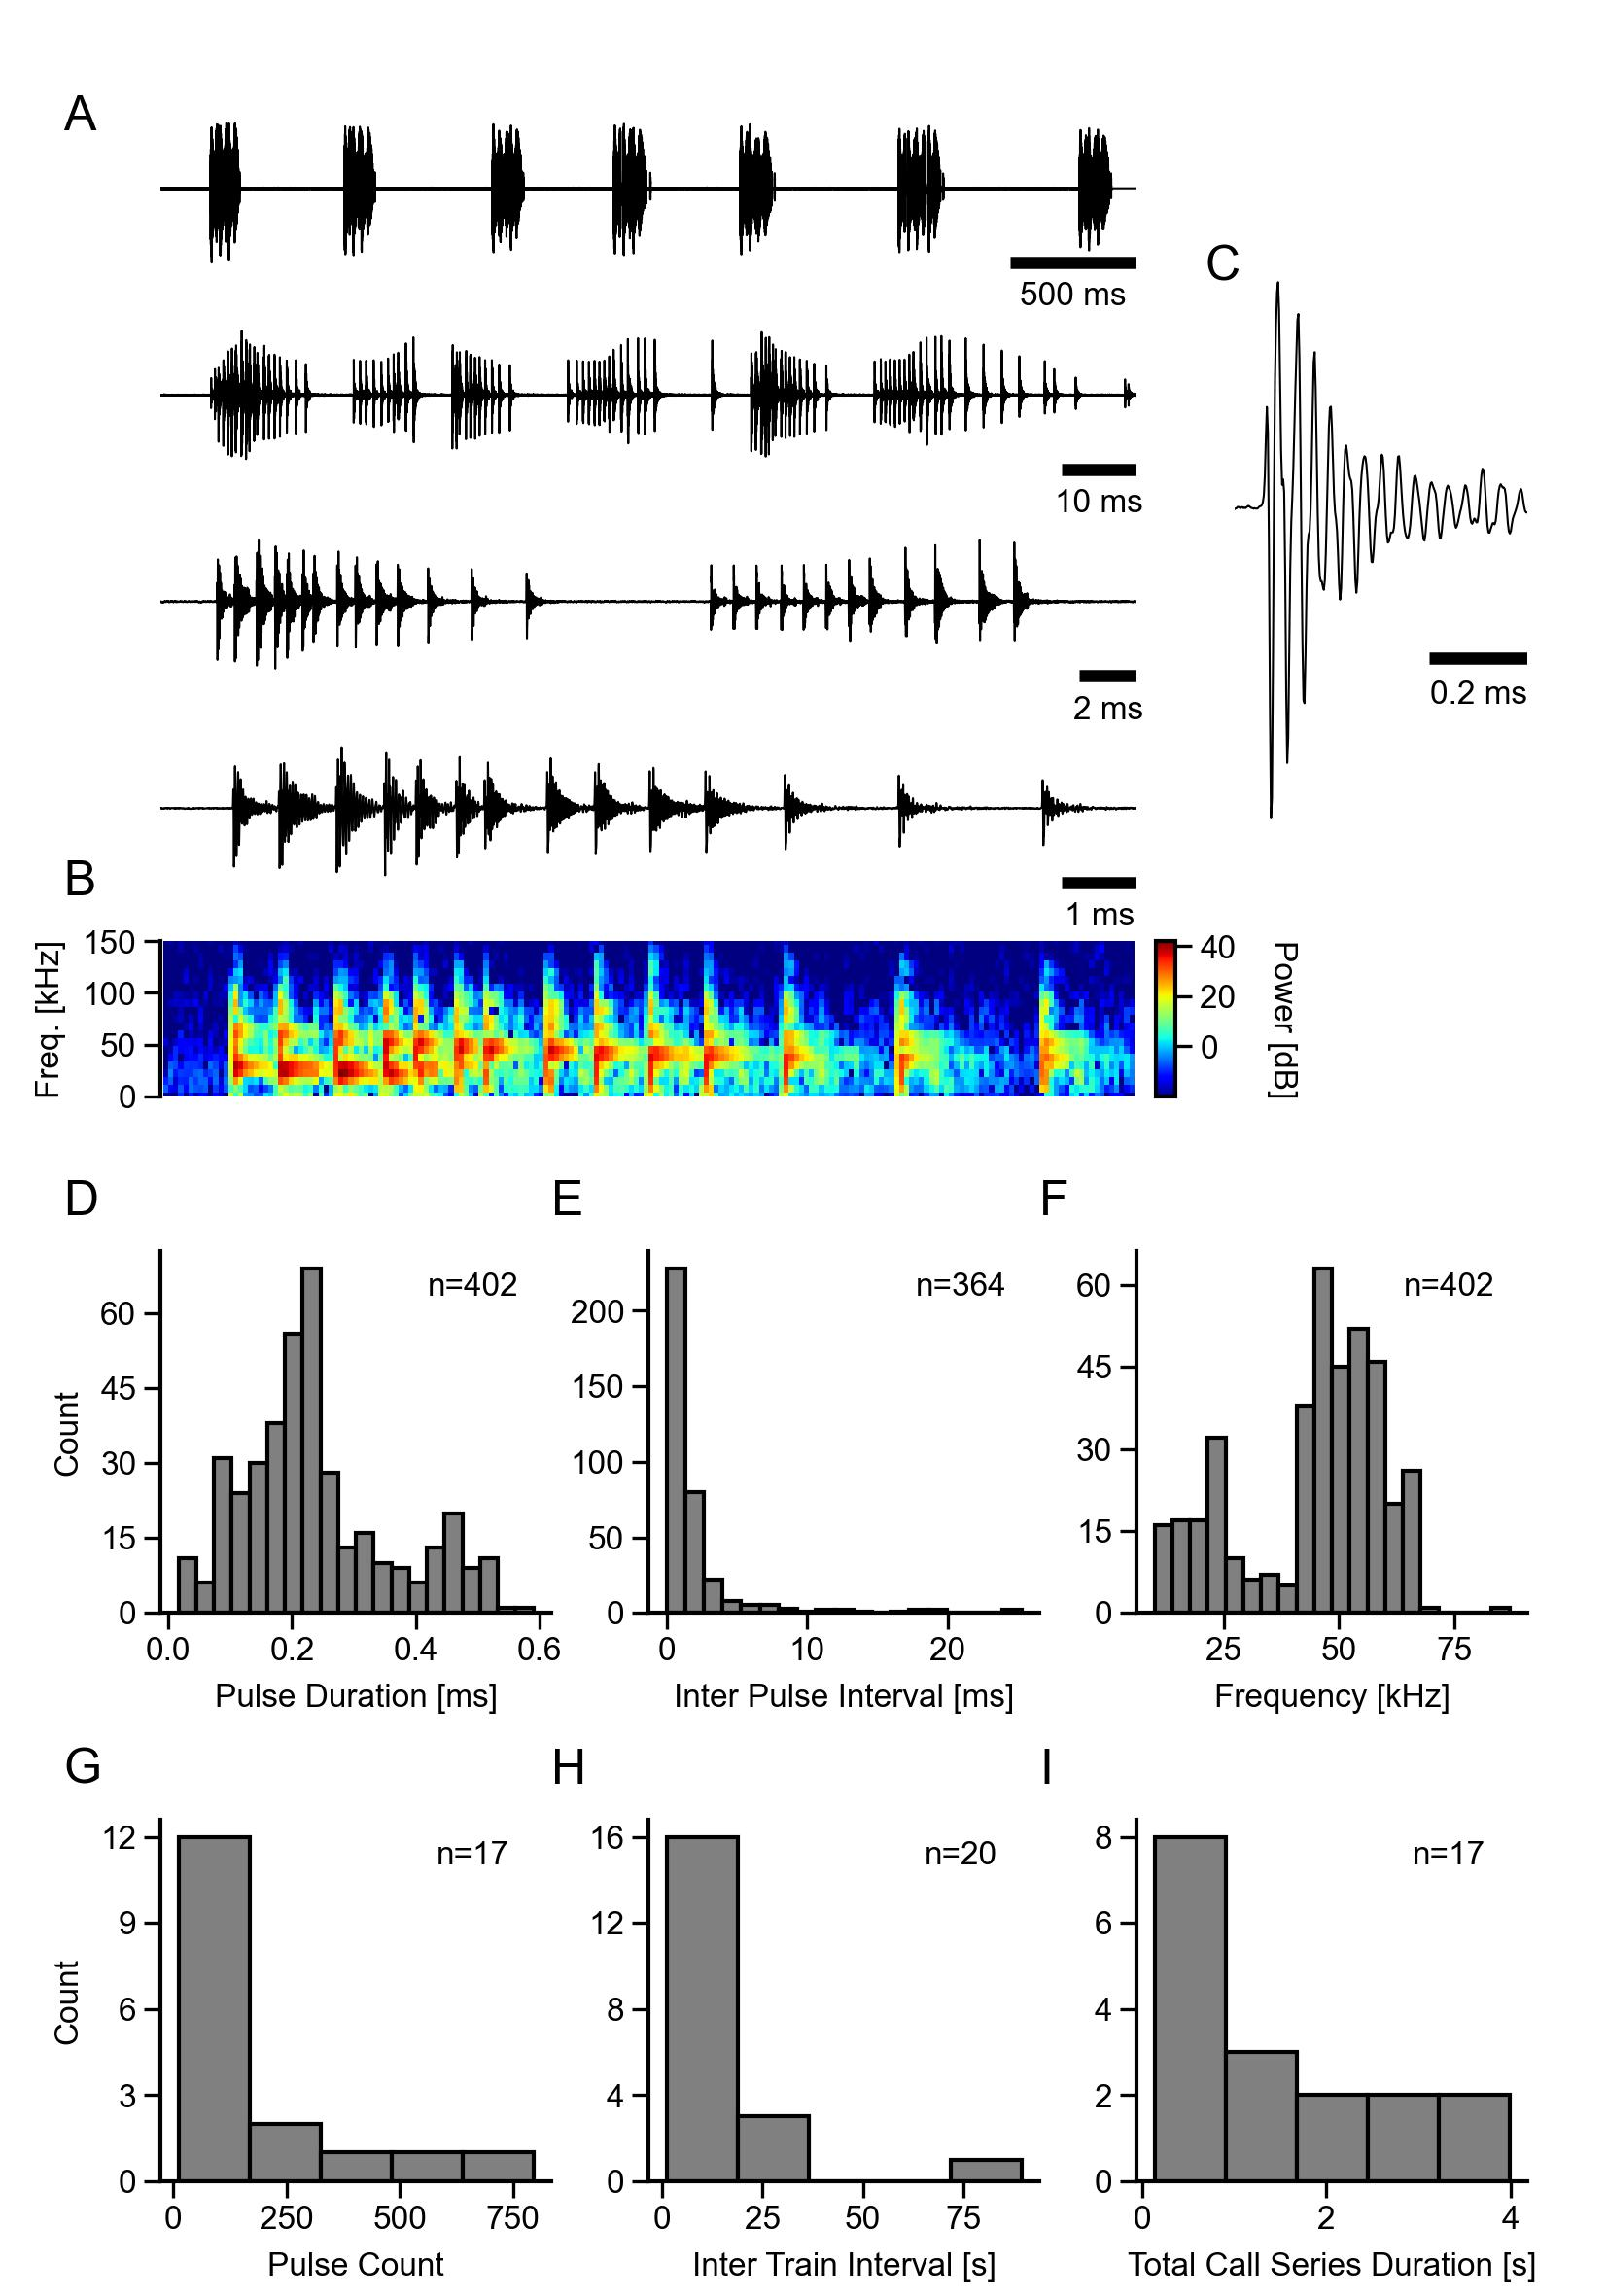
\includegraphics{figures/Fig_01.jpeg}
    % \includesvg[width=0.75\columnwidth]{figures/Fig_01.svg}
	\caption{\label{fig:01}(A) Call structure of \species{Melese sp.}. From top bottom: Packages, package with three calls, single call, active pulse train. (B) Spectrogram of the active pulse train above. (C) Single active pulse. Scale bars in each panel indicate time in milliseconds.
    Histograms of (D) Pulse Duration, (E) Inter Pulse Interval, (F) Carrier Frequency, (G) Pulse Count, (H) Inter Train Interval and (I) Total Call Series Duration. The sample size is in each panel is indicated by n.}
\end{figure}

\begin{figure}[h!]
	\centering
	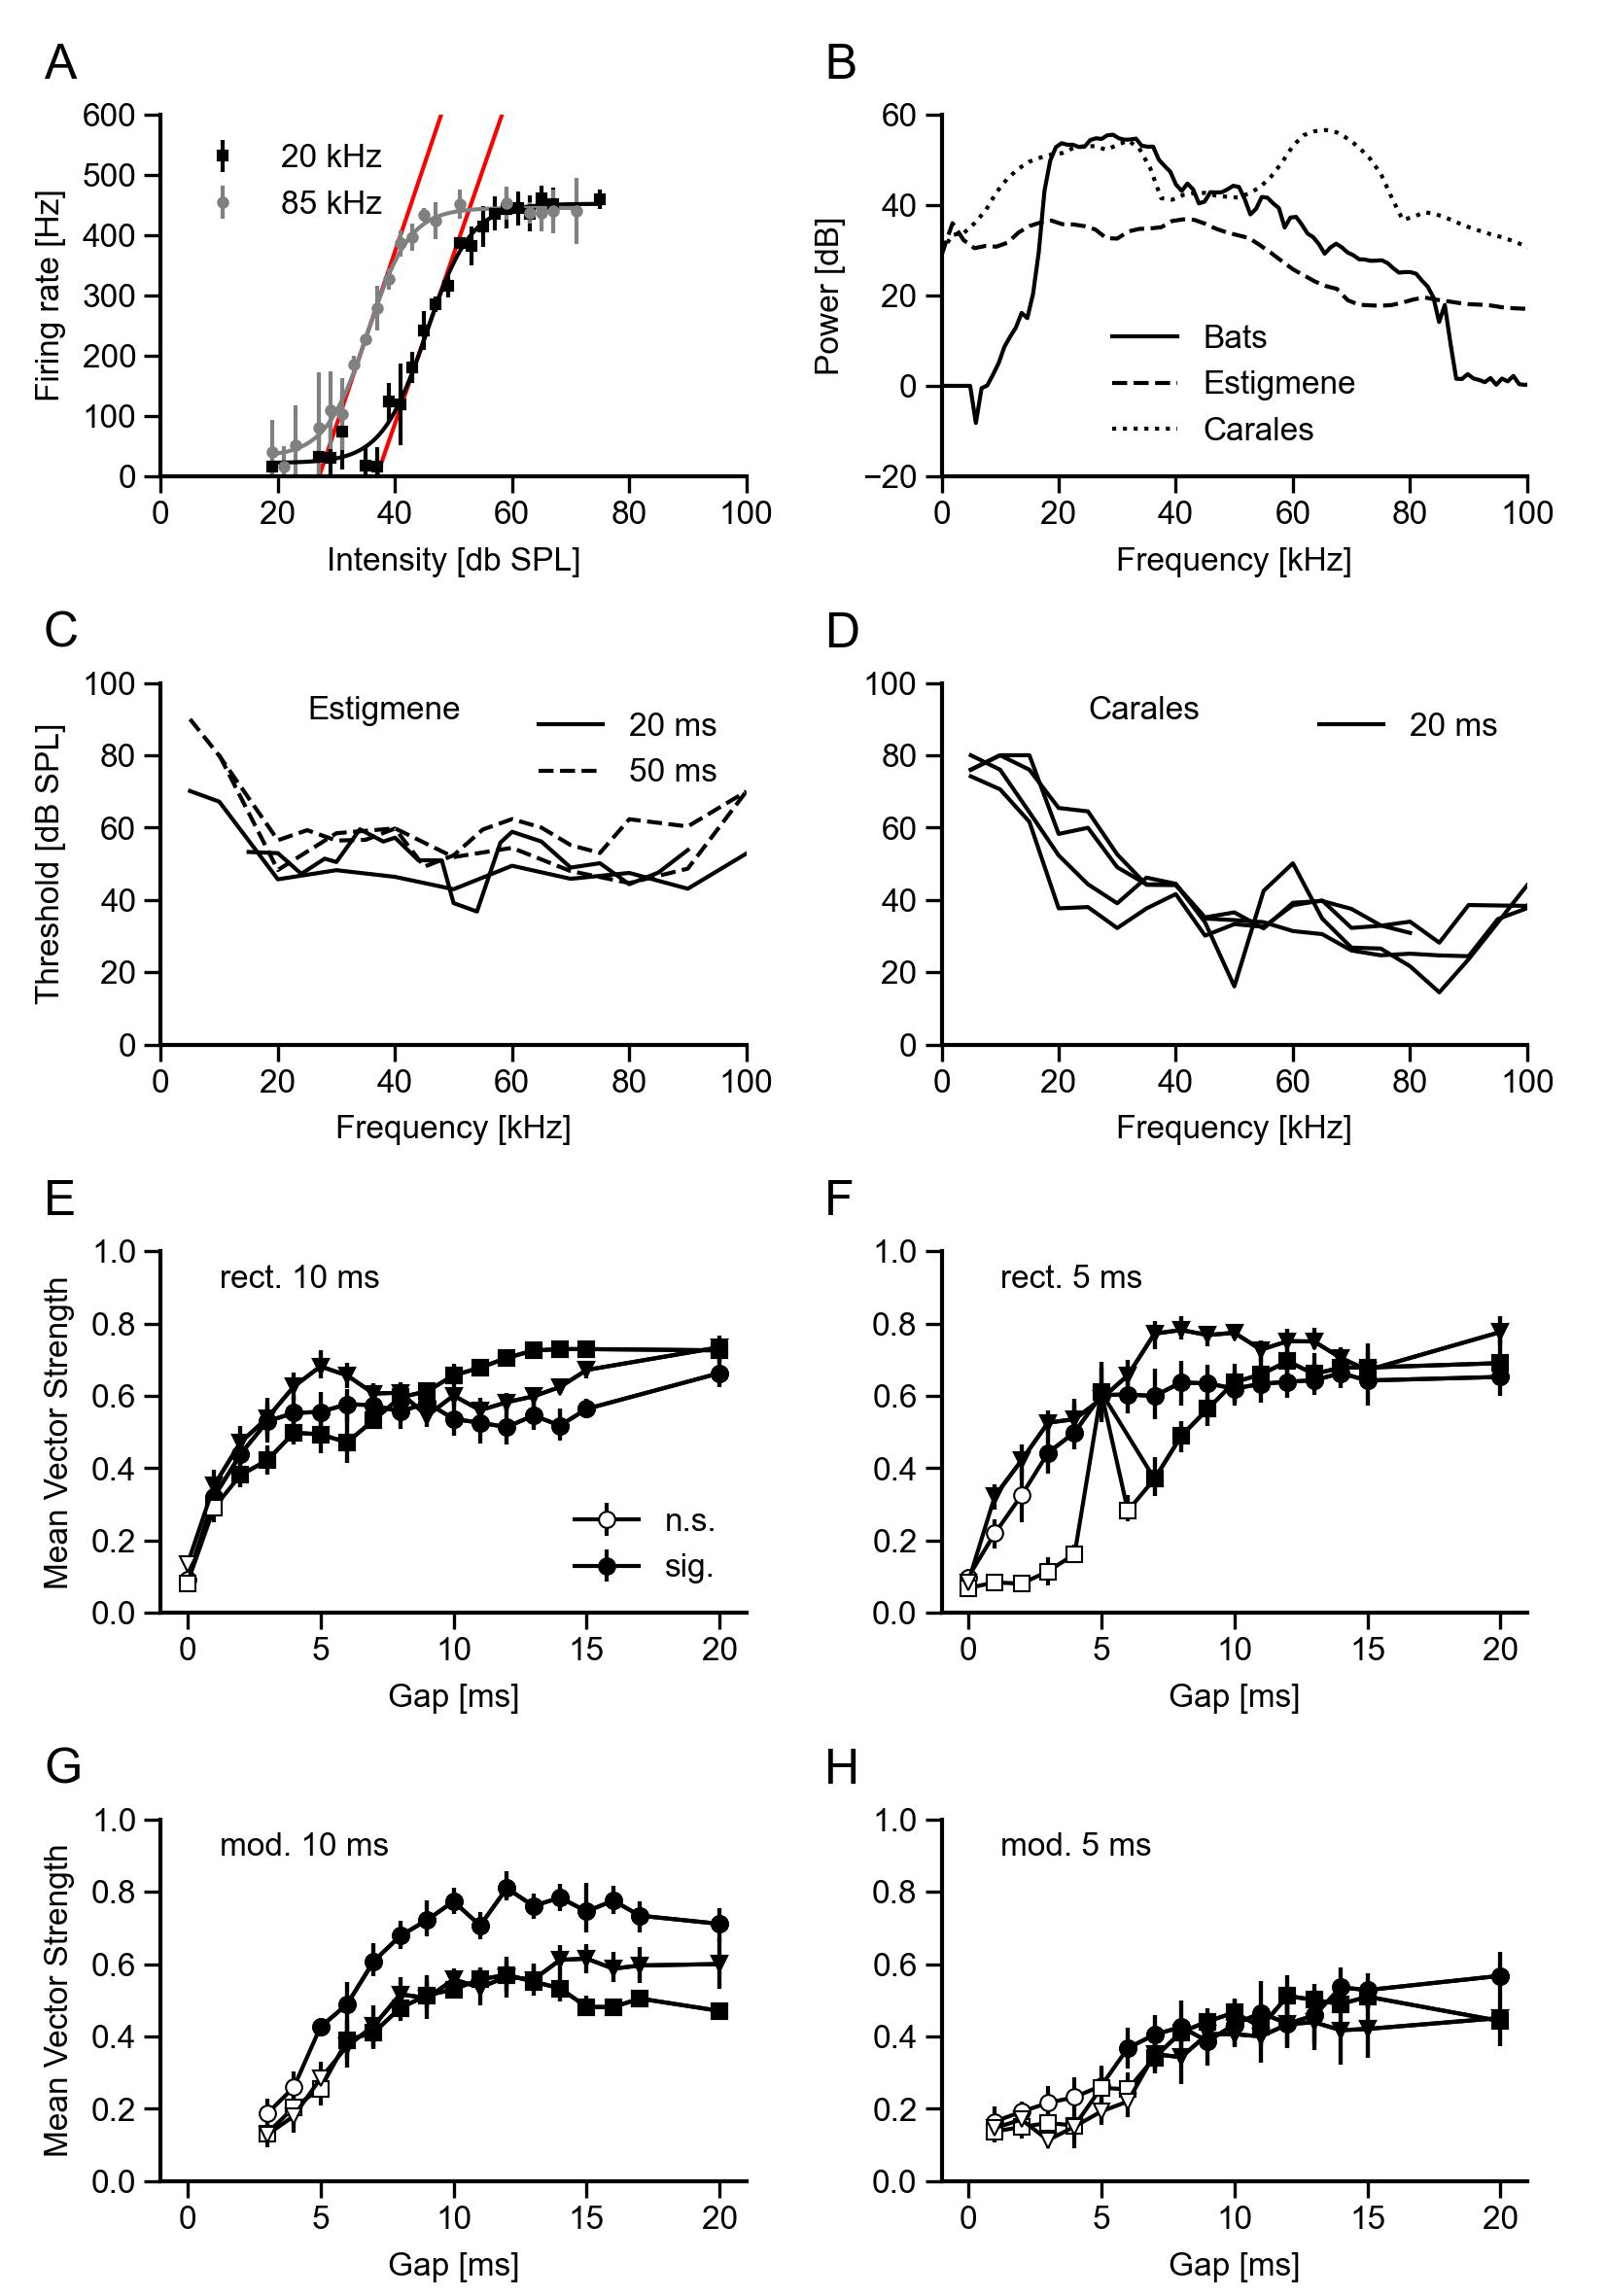
\includegraphics{figures/Fig_02.jpeg}
	\caption{\label{fig:02}(A)}
\end{figure}

\begin{figure}[h!]
	\centering
	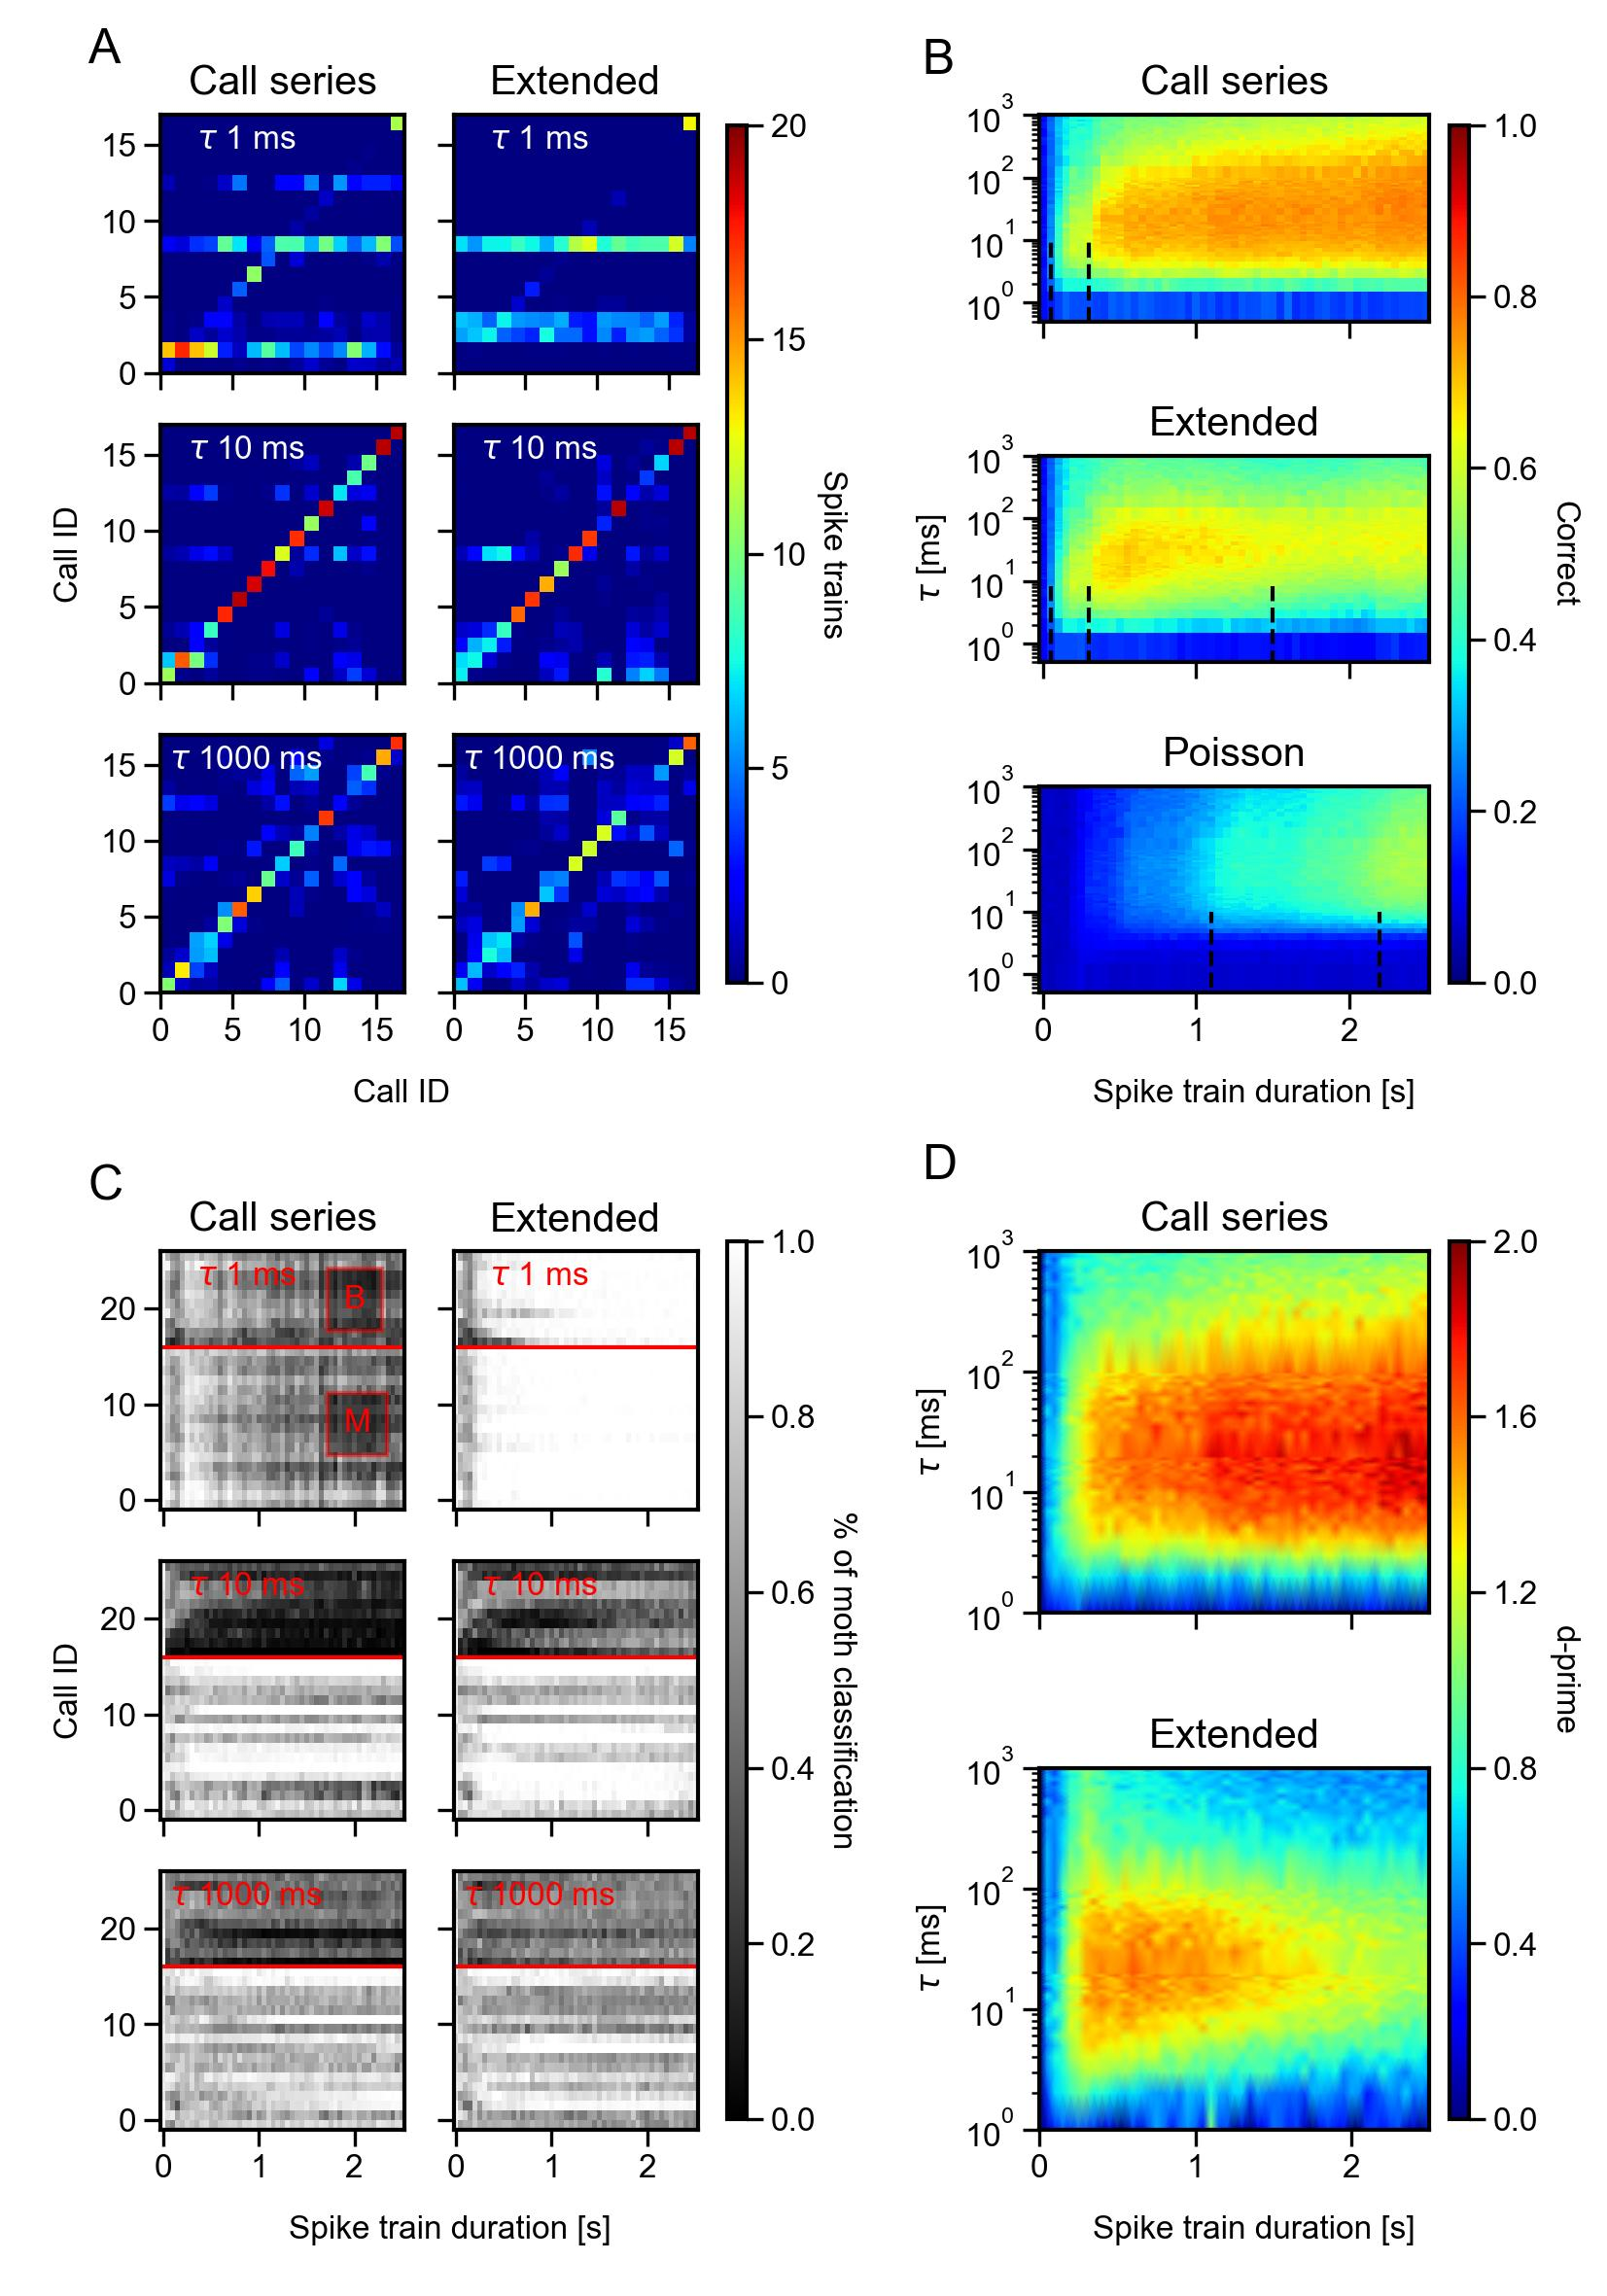
\includegraphics{figures/Fig_03.jpeg}
	\caption{\label{fig:03}(A)}
\end{figure}

\FloatBarrier
%%%%%%%%%%%%%%%%%%%%%%%%%%%%%%%%%%%%%%%%%%%%%%%%%%%%%%%%%%%%
% Appendix
%%%%%%%%%%%%%%%%%%%%%%%%%%%%%%%%%%%%%%%%%%%%%%%%%%%%%%%%%%%%
\newpage
\section*{Appendix}
\end{document}